% Provenance (never printed): see sources/outline_sources.md (Year 3:
% ocean dynamics: the Ekman layer derived, the Sverdrup balance, western
% intensification, the abyssal circulation, ocean tides).
% Brief: sources/book5/BRIEFS.md, ch. 21. Curves from
% figdata/bachelor-3/wind_driven_gyre.py and tides.py. Exercise and problem
% values in the Book 5 scratch calculator calc/ch21.py. The basins, winds
% and stations of the exercises and the problem are invented.
\chapter{महासागर गतिकी}\label{ch:b3:ocean-dynamics}

फ़्लोरिडा जलडमरूमध्य से होकर खाड़ी धारा लगभग
\qty{32}{\sverdrup} जल उत्तर की ओर ले जाती है, और तट के साथ-साथ चलते हुए उसकी मात्रा बढ़ती जाती है,
लगभग \qty{150}{\sverdrup} तक, \ang{40} N के निकट पहुँचती है। उसी महासागर की दूसरी ओर, पुर्तगाल और उत्तरी अफ़्रीका के
सामने कुछ भी वैसा दक्षिण की ओर नहीं बहता: खाड़ी धारा जो जल उत्तर ले जाती है
वह भूमध्य रेखा की ओर धीमे, चौड़े प्रवाह के रूप में लौटता है, जो हज़ारों
किलोमीटर खुले समुद्र में फैला है। उत्तरी गोलार्ध की हर महासागरीय द्रोणी में
वही असममित आकार होता है, जिसकी तेज़ धारा पश्चिमी पार्श्व पर होती है।
इस असममिति का कारण पवन, समुद्र का घर्षण और पृथ्वी का एक तथ्य है:
कोरिऑलिस प्राचल ध्रुव की ओर बढ़ता है।
% ledger: rapid:transports (31.7 Sv, rounded), stewart:north-atlantic

\begin{recall}
चंद्रमा और सूर्य का ज्वारीय बल, वृहत् और लघु ज्वार, भौतिकी की
पुस्तकों में हैं। पवन प्रतिबल, एकमन परत, एकमन परिवहन और
एकमन सर्पिल, उत्स्रवण और अवस्रवण, वलय, पश्चिमी
सीमा धाराएँ, स्वेर्द्रुप ($\qty{1}{\sverdrup} =
\qty{e6}{m^3/s}$), याम्योत्तर पलट परिसंचरण और
गहन जल का निर्माण पुस्तक 3 (स्नातक वर्ष 1) में है, उसके महासागर
परिसंचरण वाले अध्याय में; वहाँ पवन प्रतिबल $\vec T$ लिखा गया है, यहाँ
$\vec\tau$। कोरिऑलिस प्राचल, $\beta$-समतल, रॉस्बी त्रिज्या
और भू-विक्षेपी संतुलन अध्याय~\ref{ch:b3:gfd-foundations} में हैं;
भ्रमिलता और \omterm{def:b3:atmospheric-dynamics:pv}{विभव भ्रमिलता} अध्याय~\ref{ch:b3:atmospheric-dynamics} में।
\end{recall}

\section{एकमन परत की व्युत्पत्ति}\label{sec:b3:ocean-dynamics:ekman}

पुस्तक 3 (स्नातक वर्ष 1) में एकमन परिवहन पूरी परत पर बलों के संतुलन से ज्ञात किया गया था,
और उसके भीतर वेगों के सर्पिल का केवल कथन किया गया था। अचर भँवर श्यानता
$A_z$ वाले विक्षुब्ध घर्षण में सर्पिल
समीकरणों से कुछ पंक्तियों में निकलता है। क्षैतिज वेग को एक
सम्मिश्र संख्या $W = u + \mathrm iv$ और पवन प्रतिबल $\tau =
\tau_x + \mathrm i\tau_y$ के रूप में लिखा जा सकता है; $-\mathrm i$ से गुणा करने पर एक सदिश
\ang{90} दक्षिणावर्त घूमकर, ऊपर से देखने पर अपनी दाईं ओर आ जाता है।

\begin{theorem}[स्थिर पवन-चालित सतही परत की वेग-रूपरेखा]\label{thm:b3:ocean-dynamics:ekman}
स्थिर, क्षैतिज रूप से एकसमान और अत्यधिक गहरे महासागर में, जिसका अचर
घनत्व $\rho$ है, अचर ऊर्ध्वाधर भँवर श्यानता $A_z$ के साथ और कोरिऑलिस
प्राचल $f > 0$ पर, पवन प्रतिबल $\tau$ द्वारा चालित धारा निम्न होती है:
\[
W(z) = W_0\,\mathrm e^{(1+\mathrm i)z/\delta},\qquad
W_0 = \frac{\tau}{\rho\sqrt{fA_z}}\,\mathrm e^{-\mathrm i\pi/4},\qquad
\delta = \sqrt{\frac{2A_z}{f}} ,
\]
$z \le 0$ के लिए। सतही धारा प्रतिबल की दाईं ओर \ang{45} घूम जाती है;
गहराई के साथ वह और दाईं ओर मुड़ती है और $\mathrm
e^{z/\delta}$ के रूप में क्षय होती है; कुल परिवहन $\int_{-\infty}^0 W\,\mathrm dz =
-\mathrm i\tau/(\rho f)$ प्रतिबल की दाईं ओर के समकोण पर होता है।
\end{theorem}

\begin{proof}
तट से दूर परत में कोई क्षैतिज दाब-प्रवणता नहीं होती,
और कोरिऑलिस बल घर्षण को संतुलित करता है: $-fv = A_z u''$ और $fu =
A_z v''$, जहाँ प्राइम $z$ के सापेक्ष अवकलज हैं। दूसरे समीकरण को
$\mathrm i$ से गुणा करके और जोड़ने पर $A_zW'' = \mathrm ifW$ मिलता है। इसके हल हैं
$\mathrm e^{\pm(1+\mathrm i)z/\delta}$, क्योंकि $(1+\mathrm i)^2/\delta^2 =
2\mathrm i/\delta^2 = \mathrm if/A_z$; केवल धन चिह्न वाला हल
$z \to -\infty$ पर परिबद्ध रहता है। सतह पर प्रतिबल घर्षण द्वारा वहन होता है,
$\rho A_zW'(0) = \tau$, अतः $W_0 = \tau\delta/(\rho A_z(1+\mathrm i))$।
चूँकि $\delta/(\sqrt2 A_z) = 1/\sqrt{fA_z}$ और $1/(1+\mathrm i) = \mathrm
e^{-\mathrm i\pi/4}/\sqrt2$, यह कथित $W_0$ है। गुणक
$\mathrm e^{\mathrm iz/\delta}$, $z$ के घटने पर दक्षिणावर्त घूमता है। अंत में
$\int_{-\infty}^0 W\,\mathrm dz = W_0\delta/(1+\mathrm i) =
\tau\delta^2/(\rho A_z(1+\mathrm i)^2) = \tau\delta^2/(2\mathrm i\rho A_z)
= -\mathrm i\tau/(\rho f)$।
\end{proof}

यह प्रमेय पुस्तक 3 (स्नातक वर्ष 1) के दोनों परिणाम पुनः प्राप्त करता है: एकमन की सतही
धारा \ang{45} पर, और परिवहन $\tau/(\rho f)$ जो प्रतिबल के समकोण पर होता है,
और $A_z$ से स्वतंत्र है, जो कभी भली-भाँति ज्ञात नहीं होता।
$\pi\delta$ गहराई पर धारा सतही धारा के विपरीत बहती है और उसका परिमाण
$\mathrm e^{-\pi}$ गुना घटकर \qty{4}{\percent} रह जाता है।

\begin{definition}[एकमन गहराई; एकमन पंपन]\label{def:b3:ocean-dynamics:ekman-pumping}
\emph{एकमन गहराई}\index{एकमन गहराई} $D_E = \pi\delta =
\pi\sqrt{2A_z/f}$ है, वह गहराई जिस पर एकमन सर्पिल की धारा
सतही धारा के विपरीत बहती है; यह
एकमन परत की मोटाई मापती है। \emph{एकमन पंपन}\index{एकमन पंपन} वह ऊर्ध्वाधर
वेग $w_E$ है, जो एकमन परत के आधार पर एकमन परिवहन के अभिसरण या
अपसरण से प्रेरित होता है: जहाँ परिवहन अभिसरित होते हैं, वहाँ नीचे की ओर;
और जहाँ वे अपसरित होते हैं, वहाँ ऊपर की ओर, जिसे कभी एकमन चूषण कहते हैं।
\end{definition}

\begin{proposition}[एकमन पंपन]\label{prop:b3:ocean-dynamics:pumping}
समुद्र की सतह पर ऊर्ध्वाधर वेग शून्य होने पर, \omterm{def:b3:ocean-dynamics:ekman-pumping}{एकमन पंपन} निम्न होता है:
\[
w_E = \operatorname{curl}_z\frac{\vec\tau}{\rho f}
= \frac{1}{\rho f}\Big(\frac{\partial\tau_y}{\partial x} -
\frac{\partial\tau_x}{\partial y}\Big) + \frac{\beta\tau_x}{\rho f^2} ,
\]
ऊपर की ओर धनात्मक।
\end{proposition}

\begin{proof}
परत का आयतन परिवहन $(U_E, V_E) = (\tau_y,
-\tau_x)/(\rho f)$ है, जो प्रमेय का घटकों में लिखा रूप है। परत के आर-पार
सातत्य समीकरण $\partial w/\partial z = -(\partial u/\partial x +
\partial v/\partial y)$ का समाकलन करने पर, $w(0) - w_E = -(\partial
U_E/\partial x + \partial V_E/\partial y)$, तो $w_E = \partial_x(\tau_y/\rho
f) - \partial_y(\tau_x/\rho f)$। विस्तार करते समय $\mathrm df/\mathrm dy =
\beta$ रखा जाता है, और दूसरा रूप प्राप्त होता है।
\end{proof}

समुद्र के ऊपर चक्रवाती दिशा में घूमने वाली पवन, जिसका कर्ल धनात्मक है,
परत के नीचे से जल ऊपर खींचती है; प्रतिचक्रवाती पवन उसे नीचे धकेलती है। उपोष्णकटिबंधीय
महासागरों पर व्यापारिक पवनें भूमध्य रेखा वाले पक्ष पर पूर्व से बहती हैं,
और पछुआ पवनें ध्रुव वाले पक्ष पर पश्चिम से। उनके एकमन परिवहन
व्यापारिक पवनों के नीचे उत्तर की ओर, और पछुआ पवनों के नीचे दक्षिण की ओर,
दोनों के बीच अभिसरित होते हैं: पृष्ठीय जल जमा होता है और नीचे की ओर पंपित होता है, जैसा
नीचे दिए चित्र में है। किसी तट के किनारे, जहाँ
पवन तट को अपनी बाईं ओर रखकर बहती है (उत्तरी गोलार्ध में), तो
परिवहन तट से दूर जाता है, और पुस्तक 3 (स्नातक वर्ष 1) का तटीय उत्स्रवण
एक दीवार के विरुद्ध संकेंद्रित एकमन चूषण है।

\begin{omfigure}
\centering
\begin{tikzpicture}[>=stealth, font=\small, x=1.1cm, y=1cm]
\fill[omThm!7] (-5,0) rectangle (5,-3.6);
\draw[thick] (-5,0) -- (5,0);
\draw[black!45, densely dashed] (-5,-0.9) -- (5,-0.9);
\node[font=\scriptsize, black!60, anchor=north east, inner sep=1pt] at (4.95,-0.95) {एकमन परत};
% winds: west is out of the page, east into the page
\foreach \x in {-4.2,-3.4,-2.6} {\draw (\x,0.55) circle (0.13); \fill (\x,0.55) circle (0.04);}
\foreach \x in {2.6,3.4,4.2} {\draw (\x,0.55) circle (0.13);
  \draw (\x-0.09,0.46) -- (\x+0.09,0.64); \draw (\x-0.09,0.64) -- (\x+0.09,0.46);}
\node[above] at (-3.4,0.75) {व्यापारिक पवनें, पूर्व से};
\node[above] at (3.4,0.75) {पछुआ पवनें, पश्चिम से};
% Ekman transports converge
\draw[->, omDef, very thick] (-4.5,-0.45) -- (-1.2,-0.45);
\draw[->, omDef, very thick] (4.5,-0.45) -- (1.2,-0.45);
\node[omDef, font=\scriptsize, fill=omThm!7, inner sep=1pt] at (-2.85,-0.72) {एकमन परिवहन};
% pumping
\foreach \x in {-0.6,0,0.6} \draw[->, omThm, thick] (\x,-0.55) -- (\x,-1.55);
\node[omThm, font=\scriptsize, anchor=west] at (0.75,-1.25) {$w_E < 0$};
% squashed column and Sverdrup flow
\draw[thick, black!70] (-0.62,-1.75) rectangle (0.62,-3.1);
\node[font=\scriptsize, black!70, align=center] at (0,-2.42) {स्तंभ\\दबा हुआ};
\draw[->, omMeth, very thick] (-0.75,-2.42) -- (-3.2,-2.42);
\node[omMeth, font=\scriptsize, align=center, above] at (-2.6,-2.40) {स्वेर्द्रुप प्रवाह,\\भूमध्य रेखा की ओर};
\draw[black!45, densely dashed] (-5,-3.3) -- (5,-3.3);
\node[font=\scriptsize, black!60, anchor=south east, inner sep=1pt] at (4.95,-3.28) {पवन-चालित प्रवाह का आधार};
\node[below, font=\scriptsize] at (-5,-3.6) {दक्षिण};
\node[below, font=\scriptsize] at (5,-3.6) {उत्तर};
\end{tikzpicture}

\par\smallskip{\small उत्तरी गोलार्ध के एक उपोष्ण वलय का उत्तर--दक्षिण काट,
पूर्व पृष्ठ के भीतर की ओर। व्यापारिक पवनों और पछुआ पवनों के नीचे एकमन परिवहन
अभिसरित होते हैं, जल नीचे की ओर पंपित होता है, और नीचे के स्तंभ, दबकर,
भूमध्य रेखा की ओर खिसकते हैं, जहाँ $f$ छोटा है,
अपनी \omterm{def:b3:atmospheric-dynamics:pv}{विभव भ्रमिलता} बनाए रखने के लिए।}\label{fig:b3:ocean-dynamics:pumping}
\end{omfigure}

\section{स्वेर्द्रुप संतुलन}\label{sec:b3:ocean-dynamics:sverdrup}

एकमन परत के नीचे महासागर भू-विक्षेपी होता है। जल का एक स्तंभ, जो
\omterm{def:b3:ocean-dynamics:ekman-pumping}{एकमन पंपन} से दबा हुआ है, \omterm{def:b3:atmospheric-dynamics:pv}{विभव भ्रमिलता} $f/h$ बनाए रखने के लिए
जहाँ $f$ छोटा है, उस ओर, यानी भूमध्य रेखा की ओर, खिसकना होगा। 1947 में एच.~यू.~स्वेर्द्रुप
ने पवन-चालित प्रवाह की संपूर्ण गहराई के लिए इस तर्क को परिमाणात्मक बनाया।
% ledger: stewart:ekman-layer (Sverdrup 1947)

\begin{theorem}[स्वेर्द्रुप संतुलन]\label{thm:b3:ocean-dynamics:sverdrup}
एक स्थायी महासागर में, जिसमें अरेखीय पद और पार्श्व घर्षण
नगण्य हैं, एकमन परत के नीचे का आंतरिक भाग भू-विक्षेपी है, और
किसी गहराई $-H$ पर ऊर्ध्वाधर वेग शून्य हो, तो
पवन-चालित प्रवाह की प्रति इकाई चौड़ाई पर कुल उत्तरमुखी आयतन परिवहन
\emph{स्वेर्द्रुप संतुलन}\index{स्वेर्द्रुप संतुलन} का पालन करता है:
\[
\beta V = \frac{1}{\rho}\operatorname{curl}_z\vec\tau
= \frac{1}{\rho}\Big(\frac{\partial\tau_y}{\partial x} -
\frac{\partial\tau_x}{\partial y}\Big) .
\]
\end{theorem}

\begin{proof}
भू-विक्षेपी आंतरिक भाग में $fv_g = \rho^{-1}\partial p/\partial x$ और
$fu_g = -\rho^{-1}\partial p/\partial y$। अतः $\partial_x(fu_g) +
\partial_y(fv_g) = 0$, अर्थात् $f(\partial_xu_g + \partial_yv_g) + \beta
v_g = 0$ है, और सातत्य के साथ $\beta v_g = f\,\partial w/\partial z$।
$-H$ से, जहाँ $w = 0$ है, एकमन परत के आधार तक समाकलन करने पर
जहाँ $w = w_E$ है, $\beta V_g = fw_E$ प्राप्त होता है।
\cref{prop:b3:ocean-dynamics:pumping} से, $fw_E = \rho^{-1}\operatorname{curl}_z
\vec\tau + \beta\tau_x/(\rho f)$। एकमन परिवहन $V_E =
-\tau_x/(\rho f)$ को $\beta$ से गुणा करके जोड़ने पर अंतिम पद निरस्त हो जाता है:
$\beta(V_g + V_E) = \rho^{-1}\operatorname{curl}_z\vec\tau$।
\end{proof}

यह संतुलन इस बात में उल्लेखनीय है कि इसे किन चीज़ों की ज़रूरत नहीं पड़ती: न प्रवाह की
गहराई, न उसकी ऊर्ध्वाधर संरचना, न भँवर श्यानता, केवल पवन का
कर्ल और $\beta$। स्वेर्द्रुप ने इसे गति के समीकरणों से निकाला, जिन्हें
गति-रहित गहराई तक समाकलित किया गया था, और इसका परीक्षण पूर्वी उष्णकटिबंधीय प्रशांत महासागर में
अनुसंधान पोतों \emph{कार्नेगी} और
\emph{बुशनेल} के हाइड्रोग्राफ़िक खंडों से किया, \ang{34} N और
\ang{10} S के बीच, \qty{1000}{m} पर गति-रहित गहराई रखकर: पवन से परिकलित परिवहन,
घनत्व क्षेत्र से परिकलित परिवहनों से मेल खाते थे, यहाँ तक कि जहाँ धाराएँ
पवन के विपरीत बहती थीं। बेहतर पवनों के साथ बाद के कार्य में
\qty{500}{m} के आसपास की गति-रहित गहराई पर सर्वोत्तम मेल मिला, और
1999 में भूमध्यरेखीय प्रशांत महासागर में माध्य प्रतिबल के मापनों ने वहाँ
के प्रवाह को \omterm{thm:b3:ocean-dynamics:sverdrup}{स्वेर्द्रुप संतुलन} में पाया। यह संतुलन हर जगह लागू होता है या नहीं,
यह दिखाना इसे मान लेने से कठिन है: लगभग हर महासागरीय परिसंचरण सिद्धांत
इसी से आरंभ होता है।
% ledger: stewart:sverdrup

इस अध्याय की समस्या की काल्पनिक द्रोणी मान लीजिए: \ang{20} और
\ang{50} N के बीच, \qty{6000}{km} चौड़ी, पूर्व-पश्चिमी प्रतिबल $\tau_x =
-\tau_0\cos(\pi(\varphi - \ang{20})/\ang{30})$ के अंतर्गत, $\tau_0 =
\qty{0.1}{Pa}$, \ang{20} N पर पूर्वी, \ang{50} N पर पश्चिमी और
\ang{35} N पर शून्य। लगभग पूरी द्रोणी में प्रतिबल कर्ल ऋणात्मक है:
जल नीचे की ओर पंपित होता है, \ang{35} N पर लगभग \qty{35}{m} प्रति वर्ष, और
आंतरिक भाग दक्षिण की ओर बहता है, \ang{35} N पर प्रति मीटर चौड़ाई \qty{4.9}{m^2/s},
पूरी द्रोणी में \qty{29.4}{\sverdrup}। प्रेक्षित पवनों से परिकलित,
उत्तरी अटलांटिक उपोष्ण वलय का स्वेर्द्रुप परिवहन लगभग
\ang{28} N के पास \qty{30}{\sverdrup} तक पहुँचता है।
% ledger: stewart:north-atlantic (computed in figdata/bachelor-3/wind_driven_gyre.py)

\begin{omfigure}
\begin{tikzpicture}
\begin{groupplot}[group style={group size=3 by 1, horizontal sep=0.45cm, yticklabels at=edge left},
  width=0.37\linewidth, height=0.46\linewidth, ymin=20, ymax=50, ytick={20,25,30,35,40,45,50},
  tick label style={font=\scriptsize}, label style={font=\small}, title style={font=\small}]
\nextgroupplot[xlabel={$\tau_x$ (\unit{Pa})}, ylabel={अक्षांश (\unit{\degree} N)},
  xmin=-0.12, xmax=0.12, xtick={-0.1,0,0.1}, title={पवन प्रतिबल},
  scaled x ticks=false, xticklabel style={/pgf/number format/fixed}]
% computed in figdata/bachelor-3/wind_driven_gyre.py
\addplot[black!50, thin] coordinates {(0,20) (0,50)};
\addplot[omThm, thick] table[x=tau, y=lat] {figdata/out/bachelor-3-wind_driven_gyre-merid.dat};
\nextgroupplot[xlabel={$w_E$ (\unit{m/yr})}, xmin=-45, xmax=12, xtick={-40,-20,0},
  title={एकमन पंपन}]
\addplot[black!50, thin] coordinates {(0,20) (0,50)};
\addplot[omDef, thick] table[x=wE, y=lat] {figdata/out/bachelor-3-wind_driven_gyre-merid.dat};
\nextgroupplot[xlabel={परिवहन (\unit{\sverdrup})}, xmin=-32, xmax=10, xtick={-30,-20,-10,0,10},
  title={स्वेर्द्रुप}]
\addplot[black!50, thin] coordinates {(0,20) (0,50)};
\addplot[omMeth, thick] table[x=Vtot, y=lat] {figdata/out/bachelor-3-wind_driven_gyre-merid.dat};
\end{groupplot}
\end{tikzpicture}

\par\smallskip{\small समस्या की काल्पनिक द्रोणी, \ang{20} से
\ang{50} N तक, \qty{6000}{km} चौड़ी। बाईं ओर, पूर्व-पश्चिमी पवन प्रतिबल, पूर्व
की ओर धनात्मक। मध्य में \omterm{def:b3:ocean-dynamics:ekman-pumping}{एकमन पंपन}, ऊपर की ओर धनात्मक: जल को
\ang{47} N के दक्षिण में नीचे की ओर धकेला जाता है, दक्षिण में सबसे प्रबल, जहाँ $f$ छोटा है,
और उससे उत्तर में ऊपर खींचा जाता है। दाईं ओर, द्रोणी के पार कुल उत्तर-दिशा स्वेर्द्रुप परिवहन:
आंतरिक भाग दक्षिण की ओर बहता है, \ang{35} N पर \qty{29.4}{\sverdrup},
उत्तरी किनारे की एक पतली पट्टी को छोड़कर, जहाँ प्रतिबल कर्ल का चिह्न बदलता है।}\label{fig:b3:ocean-dynamics:sverdrup}
\end{omfigure}
% ledger: earth:Rmean, geod5:grs80-defining

स्वेर्द्रुप परिवहन हर बिंदु पर $V$ निर्धारित करता है, परंतु धारा-फलन
को सीमा-प्रतिबंध चाहिए, और याम्योत्तर भित्ति केवल एक ही प्रतिबंध ले सकती है। यदि
आंतरिक भाग पूर्वी भित्ति से होकर प्रवाह न होने का प्रतिबंध संतुष्ट करता है, तो दक्षिण-दिशा का प्रवाह
पश्चिमी भित्ति पर जाने का कोई रास्ता नहीं पाता; द्रव्यमान एक ऐसी धारा द्वारा लौटाया जाता है
जिसे घर्षण-रहित स्वेर्द्रुप समीकरण वर्णित नहीं कर सकते।

\section{पश्चिमी तीव्रीकरण}\label{sec:b3:ocean-dynamics:western}

सन् 1948 में एच.~स्टोमेल ने सबसे सरल महासागर में सबसे सरल घर्षण जोड़ा, और
पाया कि लौटता प्रवाह पश्चिमी भित्ति से सटकर सिमट जाता है, जैसा
पुस्तक 3 (स्नातक वर्ष 1) में उनके वलय के चित्र में दिखाया गया है। यह उन्होंने केवल ऐसे कोरिऑलिस
प्राचल के साथ ही पाया, जो उत्तर की ओर बढ़ता है: बिना घूर्णन के, या एकसमान घूर्णन के साथ,
उनका वलय सममित था।
% ledger: stewart:stommel, stommel:1948

\begin{definition}[पश्चिमी तीव्रीकरण; स्टोमेल मॉडल; मंक सीमा-परत]\label{def:b3:ocean-dynamics:western-intensification}
\emph{पश्चिमी तीव्रीकरण}\index{पश्चिमी तीव्रीकरण} वह स्थिति है, जिसमें
पवन-चालित वलय का लौटता प्रवाह एक सँकरी, तीव्र धारा में बदलकर
द्रोणी के पश्चिमी पार्श्व से सटकर सिमट जाता है। \emph{स्टोमेल
मॉडल}\index{स्टोमेल मॉडल} स्थिर गहराई का एक समांगी महासागर है,
आयताकार द्रोणी में, जिसे पूर्व-पश्चिमी पवन प्रतिबल चलाता है और जो
गहराई-समाकलित वेग के समानुपाती तल-घर्षण से मंद होता है, जिसकी दर $r$ है;
इसका परिवहन धारा-फलन $\psi$ ($U = -\partial\psi/\partial y$, $V =
\partial\psi/\partial x$) इस समीकरण का पालन करता है
\[
r\nabla^2\psi + \beta\frac{\partial\psi}{\partial x} =
\frac{1}{\rho}\operatorname{curl}_z\vec\tau ,\qquad \psi = 0 \text{ भित्तियों पर।}
\]
\emph{मंक सीमा-परत}\index{मंक सीमा-परत} उसी वलय की पश्चिमी
सीमा-परत है, जब पार्श्व भँवर श्यानता $A_H$
तल-घर्षण का स्थान लेती है; इसका चौड़ाई-पैमाना $\delta_M =
(A_H/\beta)^{1/3}$।
\end{definition}

यह समीकरण \omterm{thm:b3:ocean-dynamics:sverdrup}{स्वेर्द्रुप संतुलन} है, जिसमें तल-घर्षण का कर्ल
जुड़ा है: गहराई पर समाकलित करने पर, $\beta V = \rho^{-1}\operatorname{curl}_z
\vec\tau - r\zeta_T$, जहाँ $\zeta_T = \nabla^2\psi$ परिवहन की
भ्रमिलता है।

\begin{theorem}[स्टोमेल वलय की पश्चिमी सीमा-परत]\label{thm:b3:ocean-dynamics:stommel}
एक द्रोणी $0 \le x \le X$, $0 \le y \le L$ में, जहाँ $\tau_x = -\tau_0
\cos(\pi y/L)$ और $\delta_S = r/\beta \ll X$ हो, तो स्टोमेल धारा-फलन
$\delta_S/X$ में प्रमुख कोटि तक यह है,
\[
\psi = A\sin\frac{\pi y}{L}\Big[(X - x) - X\mathrm e^{-x/\delta_S}\Big],
\qquad A = \frac{\pi\tau_0}{\rho\beta L} .
\]
आंतरिक भाग $AX\sin(\pi y/L)$ दक्षिण की ओर ले जाता है; चौड़ाई
$\delta_S$ की एक सीमा-परत पश्चिमी भित्ति के विरुद्ध उसे उत्तर की ओर लौटाती है; पूर्वी भित्ति के विरुद्ध
कोई सीमा-परत नहीं बन सकती।
\end{theorem}

\begin{proof}
प्रतिबल कर्ल $-\partial\tau_x/\partial y = -(\pi\tau_0/L)\sin(\pi
y/L)$ है। द्रोणी की चौड़ाई पर घर्षण पद
$\beta$ पद से $\delta_S/X$ के अनुपात में छोटा होता है; इसे हटाने पर \omterm{thm:b3:ocean-dynamics:sverdrup}{स्वेर्द्रुप संतुलन} शेष रहता है,
$\beta\,\partial\psi/\partial x = -(\pi\tau_0/\rho L)\sin(\pi y/L)$, जिसका $x = X$ पर शून्य होने वाला हल
$\psi_I = A\sin(\pi y/L)(X - x)$ है। यह
$x = 0$ पर शून्य नहीं होता। भित्ति के निकट $\psi$ $x$ के साथ तेज़ी से बदलता है, और
समीकरण घटकर $r\,\partial^2\psi/\partial x^2 + \beta\,\partial\psi/
\partial x = 0$ हो जाता है; सुधार के लिए इसके हल एक अचर और
$\mathrm e^{-x/\delta_S}$ हैं। यह पूर्व की ओर क्षय होता है, पश्चिमी
भित्ति से दूर: $-AX\sin(\pi y/L)\,\mathrm e^{-x/\delta_S}$ जोड़ने पर $\psi = 0$
$x = 0$ पर हो जाता है और आंतरिक भाग में कुछ नहीं बदलता। पूर्वी भित्ति पर
एक सुधार को $x = X$ से दूर, पश्चिम की ओर क्षय होना होगा, और
$\mathrm e^{-x/\delta_S}$ पश्चिम की ओर बढ़ता है: ऐसी कोई परत नहीं है, इसलिए
आंतरिक भाग को पूर्वी भित्ति से स्वयं मिलना होगा, जैसा $\psi_I$ करता है।
भित्ति और वह बिंदु जहाँ $V$ चिह्न बदलता है, उसके बीच का
उत्तर-दिशा परिवहन वहाँ $\psi$ है, जो $AX\sin(\pi y/L)$ के निकट होता है।
\end{proof}

यही परिणाम भ्रमिलता से भी प्राप्त होता है। आंतरिक भाग के ऊपर पवन हर स्तंभ को
ऋणात्मक भ्रमिलता देती है, और स्तंभ दक्षिण की ओर सरककर
छोटे $f$ की ओर जाकर उसकी भरपाई करता है। लौटते समय उत्तर की ओर वह \omterm{def:b3:atmospheric-dynamics:vorticity-kinds}{ग्रहीय भ्रमिलता} प्राप्त करता है,
और उसे खोना पड़ता है, जो केवल घर्षण ही कर सकता है।
उत्तर-दिशा की धारा में, जिसकी चाल पश्चिमी भित्ति के निकट से पूर्व की ओर घटती है, $\partial
v/\partial x < 0$ उसकी अधिकांश चौड़ाई पर है: धारा की भ्रमिलता ऋणात्मक है, और घर्षण, उसके विरुद्ध कार्य करते हुए,
वह स्तंभों को आवश्यक धनात्मक भ्रमिलता देता है। पूर्वी भित्ति के विरुद्ध उत्तर-दिशा की
धारा की भ्रमिलता धनात्मक होती, और
घर्षण गलत चिह्न को हटा देता।

\begin{omfigure}
\begin{tikzpicture}
\begin{groupplot}[group style={group size=2 by 1, horizontal sep=1.7cm},
  width=0.48\linewidth, height=0.42\linewidth, xmin=0, xmax=400,
  xlabel={पश्चिमी भित्ति से दूरी (\unit{km})},
  tick label style={font=\scriptsize}, label style={font=\small},
  legend style={font=\scriptsize, draw=none, fill=none}]
\nextgroupplot[ylabel={$V$ (\unit{m^2/s})}, ymin=-80, ymax=600, legend pos=north east,
  legend cell align=left]
% computed in figdata/bachelor-3/wind_driven_gyre.py
\addplot[omThm, thick] table[x=x, y=vS] {figdata/out/bachelor-3-wind_driven_gyre-bl.dat};
\addlegendentry{स्टोमेल, $\delta_S = \qty{53}{km}$}
\addplot[omDef, thick] table[x=x, y=vM] {figdata/out/bachelor-3-wind_driven_gyre-bl.dat};
\addlegendentry{मंक, $\delta_M = \qty{64}{km}$}
\addplot[black!50, thin, forget plot] coordinates {(0,0) (400,0)};
\nextgroupplot[ylabel={भित्ति से परिवहन (\unit{\sverdrup})}, ymin=0, ymax=36,
  legend pos=south east, legend cell align=left]
\addplot[omThm, thick] table[x=x, y=cS] {figdata/out/bachelor-3-wind_driven_gyre-bl.dat};
\addlegendentry{स्टोमेल}
\addplot[omDef, thick] table[x=x, y=cM] {figdata/out/bachelor-3-wind_driven_gyre-bl.dat};
\addlegendentry{मंक}
\addplot[black!60, densely dashed] coordinates {(0,29.4) (400,29.4)};
\addlegendentry{आंतरिक भाग, \qty{29.4}{\sverdrup}}
\end{groupplot}
\end{tikzpicture}

\par\smallskip{\small समस्या के काल्पनिक बेसिन के मध्य में पश्चिमी सीमा-परत
(\ang{35} N, \qty{6000}{km} चौड़ा)। बाईं ओर, प्रति इकाई चौड़ाई पर उत्तर-दिशा
परिवहन: स्टोमेल की परत, जिसमें तल घर्षण
$r = \qty{e-6}{s^{-1}}$ है, भित्ति से घातांकीय रूप से क्षीण होती है; मंक की परत, जिसमें
$A_H = \qty{5e3}{m^2/s}$ है और भित्ति पर कोई फिसलन नहीं, शून्य से उठती है,
लगभग \qty{80}{km} दूर शिखर बनाती है और उसके बाद एक दुर्बल दक्षिण-दिशा प्रति-धारा आती है।
दाईं ओर, भित्ति और प्रत्येक दूरी के बीच का परिवहन, उस
\qty{29.4}{\sverdrup} के सापेक्ष जिसे आंतरिक भाग दक्षिण की ओर ले जाता है: स्टोमेल की परत
दक्षिण की ओर मुड़ने से पहले \qty{27.9}{\sverdrup} जुटाती है, और मंक की धारा
प्रति-धारा से पहले \qty{33.0}{\sverdrup} जुटाती है।}\label{fig:b3:ocean-dynamics:boundary}
\end{omfigure}
% ledger: stewart:munk

$r = \qty{e-6}{s^{-1}}$ पर \ang{35} N, $\delta_S = \qty{53}{km}$ के साथ, और
उत्तर-दिशा प्रवाह भित्ति से पहले \qty{250}{km} घेरता है। वर्ष 1950 में
डब्ल्यू.~एच.~मंक ने तल घर्षण के स्थान पर एक पार्श्विक भंवर श्यानता $A_H$ रखी,
जो धारा के भीतर अपरूपण पर कार्य करती है; समीकरण में एक पद
$A_H\nabla^4\psi$ जुड़ जाता है, और पश्चिमी भित्ति के निकट संशोधन
$\mathrm e^{-x/2\delta_M}$ गुणा एक दोलन हो जाता है, $\cos(\sqrt3x/2\delta_M)$
और $\sin(\sqrt3x/2\delta_M)$। $A_H = \qty{5e3}{m^2/s}$ पर उत्तर-दिशा
धारा लगभग \qty{225}{km} चौड़ी है (चित्र के बेसिन में \qty{233}{km}),
उसके परे एक दुर्बल प्रति-धारा के साथ, एक ऐसा आकार जो खाड़ी धारा और
कुरोशियो के निकट है। स्टोमेल की परत की भाँति, धारा का परिवहन घर्षण पर
नहीं, बल्कि केवल पवन-प्रतिबल की कर्ल, बेसिन की
चौड़ाई और $\beta$ पर निर्भर करता है। अपने समय की पवनों से मंक ने
खाड़ी धारा के लिए \qty{36}{\sverdrup} और कुरोशियो के लिए \qty{39}{\sverdrup} परिकलित किए,
जो उस समय मापे गए परिवहन के लगभग आधे थे; एक बेहतर खिंचाव
गुणांक और प्रतिबल के सूक्ष्म माध्यों के साथ, \qty{32}{\sverdrup} पाया गया
खाड़ी धारा के लिए वर्ष 1978 में। मुख्यतः पनडुब्बी केबल से मापी गई
फ़्लोरिडा जलडमरूमध्य की खाड़ी धारा \qty{31.7}{\sverdrup} वहन करती आई है,
औसतन वर्ष 2004 से। धारा के नीचे की ओर वह लगभग \qty{150}{\sverdrup} तक बढ़ जाती है,
\ang{40} N के निकट, और केप हैटरस के खुले सागर में एक प्रबल पुनःपरिसंचरण, जिसे
रैखिक सिद्धांत समाहित नहीं करता, इस समझौते को बिगाड़ देता है।
% ledger: stewart:munk, rapid:transports, stewart:north-atlantic

\section{गहन परिसंचरण}\label{sec:b3:ocean-dynamics:abyssal}

गहन महासागर कुछ ही स्थानों से भरता है। पुस्तक 3 (स्नातक वर्ष 1) में, गहरा
जल वहाँ बनता है जहाँ सतही जल सुदूर उत्तरी अटलांटिक और अंटार्कटिका के चारों ओर ठंडा होकर सघन
होता है, और वह बेसिनों में उत्तरी अटलांटिक गहन जल के रूप में फैलता है,
तथा अंटार्कटिक तल जल के रूप में। 1958 और 1960 के बीच
एच.~स्टोमेल, A.~B.~एरॉन्स और A.~J.~फ़ॉलर ने पूछा कि यह कैसे फैलता है, और
इसके लिए स्वेर्द्रुप के समान भ्रमिलता तर्क का प्रयोग किया।

\begin{definition}[स्टोमेल--एरॉन्स मॉडल]\label{def:b3:ocean-dynamics:abyssal}
गहन परिसंचरण का \emph{स्टोमेल--एरॉन्स मॉडल}\index{स्टोमेल--एरॉन्स मॉडल}
मानता है कि गहरा जल कुछ थोड़े-से उच्च-अक्षांश स्रोतों पर संवहन से आपूर्त होता है,
कि वह ऊपरी महासागर में एक धीमे, एकसमान
उत्स्रवण $W_0$ द्वारा ताप-प्रवणता परत के आधार से होकर लौटता है, जो
ऊष्मा के नीचे की ओर मिश्रण से संतुलित होता है, और कि आंतरिक प्रवाह भू-विक्षेपी है
और \omterm{def:b3:atmospheric-dynamics:pv}{विभव भ्रमिलता} का संरक्षण करता है। परिसंचरण गहरी पश्चिमी सीमा
धाराओं से बंद होता है।
\end{definition}

\begin{proposition}[गहन आंतरिक भाग का ध्रुव-अभिमुख प्रवाह]\label{prop:b3:ocean-dynamics:abyssal}
\omterm{def:b3:ocean-dynamics:abyssal}{स्टोमेल--एरॉन्स मॉडल} में, समतल तल पर, गहराई-समाकलित गहन आंतरिक भाग का
उत्तर-दिशा परिवहन होता है
\[
V = \frac{f}{\beta}W_0 = a\tan\varphi\,W_0 ,
\]
दोनों गोलार्धों में ध्रुव की ओर, जब $W_0 > 0$।
\end{proposition}

\begin{proof}
भू-विक्षेपी आंतरिक भाग में $\beta v = f\,\partial w/\partial z$ होता है, जैसे \omterm{thm:b3:ocean-dynamics:sverdrup}{स्वेर्द्रुप संतुलन}
की उपपत्ति में। समतल तल से, जहाँ $w = 0$ है, समाकलन करने पर
गहन परत के शीर्ष तक, जहाँ $w = W_0$ है, $\beta V =
fW_0$ प्राप्त होता है, और $f/\beta = 2\Omega\sin\varphi\,a/(2\Omega\cos\varphi) =
a\tan\varphi$। दक्षिणी गोलार्ध में $\tan\varphi < 0$ है: प्रवाह दक्षिण की ओर है,
फिर भी ध्रुव की ओर।
\end{proof}

परिणाम सहज बोध के विपरीत है: गहन आंतरिक भाग स्रोतों की ओर बहता है,
न कि उनसे दूर। स्टोमेल और एरॉन्स ने स्वयं को आश्वस्त करने के लिए घूर्णनशील-टंकी
प्रयोग बनाए। स्रोतों का जल चलता है
पश्चिमी भित्तियों के साथ, गहरी पश्चिमी सीमा धाराओं में, जो आंतरिक भाग को पोषित करती हैं
आगे बढ़ते हुए। भूमध्य रेखा और ध्रुव के बीच के महासागर-खंड में,
जब पूरा स्रोत $S_0$ ध्रुव के निकट हो, तब पश्चिमी सीमा धारा
$2S_0\sin\varphi$ भूमध्य रेखा की ओर वहन करती है, ध्रुव पर स्रोत का दोगुना और
भूमध्य रेखा पर कुछ नहीं: $S_0$ से ऊपर का अधिशेष
आंतरिक भाग से पुनःपरिसंचरित जल है। यह मॉडल गहन परिसंचरण को मिश्रण से चालित बनाता है,
डूबने से नहीं: उत्स्रवण के बिना संवहन केवल गहन भाग को
ठंडे जल के स्थिर कुंड से भर देता। इसके पारगमन-काल स्रोतों के निकट कुछ सदियों से
लेकर उत्तरी प्रशांत महासागर में लगभग एक हज़ार वर्ष तक के हैं। वास्तविक महासागर-तल पर
कटक बेसिनों को विभाजित करते हैं, खुरदरी स्थलाकृति पर मिश्रण
प्रबल होता है, और गहन प्रवाह मॉडल की तुलना में कहीं अधिक
पूर्व-पश्चिम दिशा में होता है। इसकी स्थायी भविष्यवाणी गहरी पश्चिमी सीमा धारा है: उत्तरी
अटलांटिक में वह लगभग \qty{14}{\sverdrup} जल
\qty{2}{\celsius} पर दक्षिण की ओर लौटता है, जबकि खाड़ी धारा उष्ण जल को
उत्तर की ओर ले जाती है।
% ledger: stewart:stommel-arons, stewart:deep-circulation, stewart:heat-conveyor

\begin{omfigure}
\centering
\begin{tikzpicture}[>=stealth, font=\small, scale=0.95]
\fill[omThm!7] (0,0) -- (7,0) -- (4.2,5) -- (2.8,5) -- cycle;
\draw[thick] (0,0) -- (2.8,5) -- (4.2,5) -- (7,0);
\draw[black!45, densely dashed] (0,0) -- (7,0);
\node[below, font=\scriptsize] at (3.5,0) {भूमध्य रेखा};
\node[above, font=\scriptsize] at (3.5,5) {ध्रुव की ओर};
\fill[omThm] (3.05,4.6) circle (0.17);
\node[font=\scriptsize, anchor=west, inner sep=1pt] at (3.22,4.6) {$S_0$};
% western boundary current
\draw[->, omThm, very thick] (2.75,4.35) -- (0.35,0.25);
\node[omThm, font=\scriptsize, rotate=60.8, inner sep=1pt] at (0.85,2.45) {गहरी पश्चिमी सीमा धारा};
% interior poleward flow
\foreach \x/\y in {2.6/0.7, 3.8/0.7, 5.0/0.7, 3.1/1.7, 4.3/1.7, 3.6/2.7, 4.6/2.7} {
  \draw[->, omMeth, thick] (\x,\y) -- ++(0.15,0.65);}
% upwelling dots
\foreach \x/\y in {2.2/1.25, 3.4/1.25, 4.6/1.25, 5.6/1.25, 2.7/2.2, 3.9/2.2, 5.0/2.2, 3.3/3.2, 4.3/3.2, 3.8/3.9} {
  \draw[omDef] (\x,\y) circle (0.09); \fill[omDef] (\x,\y) circle (0.03);}
\node[omMeth, font=\scriptsize, align=left, anchor=west] at (6.45,2.6) {ध्रुव की ओर\\आंतरिक प्रवाह};
\node[omDef, font=\scriptsize, align=left, anchor=west] at (6.6,1.5) {उत्स्रवण $W_0$};
\end{tikzpicture}

\par\smallskip{\small उत्तरी गोलार्ध के महासागर के एक खंड में स्टोमेल--एरॉन्स गहन परिसंचरण,
ऊपर से देखा गया। गहन जल ध्रुव के निकट
स्रोत $S_0$ पर डूबता है, भूमध्य रेखा की ओर गहरी पश्चिमी
सीमा धारा में बहता है, और ध्रुव की ओर बहने वाले आंतरिक भाग में रिसता है,
हर जगह ताप-प्रवणता परत से होकर धीरे-धीरे ऊपर उठता है (बिंदु,
पाठक की ओर उत्स्रवण)।}\label{fig:b3:ocean-dynamics:stommel-arons}
\end{omfigure}

मॉडल का आंतरिक भाग, स्वेर्द्रुप के मॉडल की तरह, भू-विक्षेपी है, और
गहन सागर की भू-विक्षेपी धाराएँ उसी ढंग से मापी जाती हैं, जिस ढंग से
स्वेर्द्रुप ने अपनी मापी थीं: घनत्व से।

\begin{definition}[गतिक विधि]\label{def:b3:ocean-dynamics:dynamic-height}
\emph{गतिक विधि}\index{गतिक विधि} दो जल-सर्वेक्षण केंद्रों के बीच की भू-विक्षेपी धारा की गणना
दोनों पर मापे गए घनत्व से करती है, संदर्भ दाब-स्तर के सापेक्ष, जहाँ
धारा शून्य या ज्ञात मानी जाती है।
दो दाब-पृष्ठों के बीच की \omterm{def:b3:gravity-geodesy:geopotential}{भू-विभव} दूरी, $\int\alpha\,\mathrm dp$,
जहाँ $\alpha = 1/\rho$ विशिष्ट आयतन है, दो भागों में
बाँटी जाती है: एक मानक भाग, जो दोनों केंद्रों पर समान है, और
\emph{\omterm{def:b3:gravity-geodesy:geopotential}{भू-विभव} विसंगति} $\Delta\Phi$; ऊपरी पृष्ठ पर धारा,
केंद्रों $A$ और $B$ के बीच की रेखा के लंबवत्, जिनके बीच की दूरी $L$ है,
यह होती है:
\[
v = \frac{\Delta\Phi_B - \Delta\Phi_A}{fL} .
\]
\end{definition}

मौसम-विज्ञानी जैसे करते हैं, वैसे दाब को सीधे क्यों नहीं मापा जाता? एक भू-विक्षेपी
धारा \qty{10}{cm/s} की, \ang{30} पर,
\qty{7.5e-3}{Pa/m} दाब-प्रवणता चाहिए, यानी \qty{750}{Pa} का दाब-अंतर, \qty{100}{km} की दूरी पर,
जो \qty{7.4}{cm} समुद्री जल के भार के बराबर है। समुद्र-तल पर कोई दाब-मापी
इतनी बारीकी से अंशांकित नहीं की जा सकती। घनत्व, जिसे कुछ दस-लाखवें भागों तक परिकलित किया जाता है,
इसके बजाय एक दाब-पृष्ठ की दूसरे के सापेक्ष ढलान देता है। हल्का, गर्म जल
धारा की दाहिनी ओर होता है, बहाव की ओर देखने पर,
उत्तरी गोलार्ध में। खाड़ी धारा के आर-पार स्थिर घनत्व के
पृष्ठ \qty{100}{km} में एक किलोमीटर से अधिक गहराई बदलते हैं।
% ledger: stewart:dynamic-method

\begin{method}[दो केंद्रों से भू-विक्षेपी धारा]\label{met:b3:ocean-dynamics:dynamic}
\begin{enumerate}
\item हर केंद्र पर विशिष्ट-आयतन विसंगति $\delta =
  \alpha(S, T, p) - \alpha(35, 0, p)$ मापी गई लवणता,
  तापमान और दाब से परिकलित कीजिए।
\item इसे संदर्भ दाब से प्रत्येक दाब $p$ तक समाकलित कीजिए:
  $\Delta\Phi(p) = \int_p^{p_{\text{संदर्भ}}}\delta\,\mathrm dp$।
\item प्रत्येक दाब पर $v(p) = (\Delta\Phi_B - \Delta\Phi_A)/(fL)$ संदर्भ स्तर के सापेक्ष
  धारा है, जो धनात्मक होती है जब
  केंद्र $B$ दाहिनी ओर हो।
\item संदर्भ स्तर पर धारा ज्ञात हो, तो उसे जोड़िए, जो वहाँ बहते एक फ़्लोट से
  या उपग्रह द्वारा मापी गई समुद्र-पृष्ठ की ढलान से मिली हो।
\end{enumerate}
\end{method}

\begin{inthefield}[फ़्लोटों का जाल]
\begin{minipage}[t]{0.52\linewidth}\vspace{0pt}
\begin{dated}{2024}
लगभग चार हज़ार आर्गो फ़्लोट विश्व महासागर में बहते हैं। जहाज़ के किनारे से
उतारे जाने पर एक फ़्लोट लगभग \qty{1000}{m} तक डूबता है और वहाँ
लगभग नौ दिन बहता है; फिर वह \qty{2000}{m} तक डूबता है और सतह पर उठता है,
रास्ते में चालकता, तापमान और दाब मापते हुए, और चक्र लगभग हर दस दिन में फिर शुरू होता है;
गहरे आर्गो फ़्लोट \qty{6000}{m} तक प्रोफ़ाइल मापते हैं।
जुलाई 2024 में इस जाल ने अपनी तीस लाखवीं
प्रोफ़ाइल एकत्र की। इन प्रोफ़ाइलों से समुद्रविज्ञानी हर फ़्लोट पर \omterm{def:b3:ocean-dynamics:dynamic-height}{गतिक विधि} की \omterm{def:b3:gravity-geodesy:geopotential}{भू-विभव}
विसंगतियाँ परिकलित करते हैं, और दो बार सतह पर आने के बीच फ़्लोट का अपना
विस्थापन ठहराव-गहराई पर माध्य धारा देता है:
वह संदर्भ वेग जिसे स्वेर्द्रुप को मानना पड़ा था, अब मापा जाता है।
\end{dated}
\end{minipage}\hfill
\begin{minipage}[t]{0.44\linewidth}\vspace{0pt}
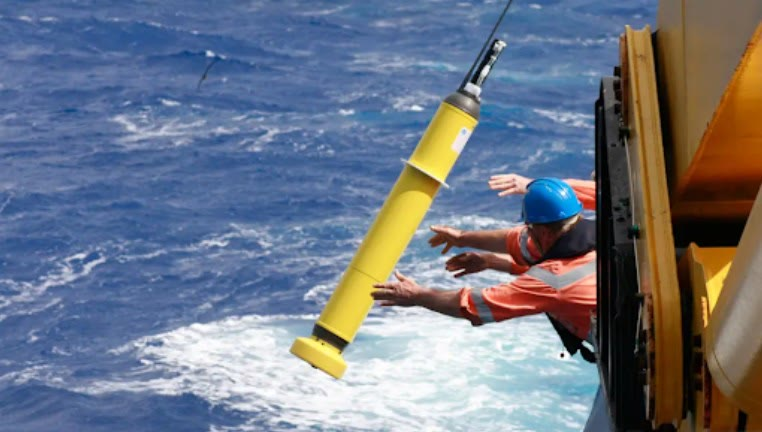
\includegraphics[width=\linewidth]{images/book5/b3-argo-deploy.jpg}

{\scriptsize अनुसंधान पोत के किनारे से उतारा गया एक आर्गो फ़्लोट (NOAA
Global Ocean Monitoring and Observing Program, सार्वजनिक डोमेन)।}
\end{minipage}
\end{inthefield}
% ledger: argo:fleet, noaa:argo-25, photo:b3-argo-deploy

\section{महासागरीय ज्वार}\label{sec:b3:ocean-dynamics:tides}

दिन में दो बार, और हर दिन लगभग एक घंटे से कुछ कम देर बाद, समुद्र उठता और
गिरता है। भौतिकी की पुस्तकें ज्वारीय बल समझाती हैं: चंद्रमा का आकर्षण
पृथ्वी के निकटवर्ती पक्ष पर उसके केंद्र की तुलना में अधिक, और
दूरवर्ती पक्ष पर कम होता है, इसलिए केंद्र के सापेक्ष जल
दोनों ओर चंद्रमा की ओर की रेखा के अनुदिश बाहर खींचा जाता है।

\begin{definition}[साम्य ज्वार; ज्वारीय घटक]\label{def:b3:ocean-dynamics:tides}
\emph{साम्य ज्वार}\index{साम्य ज्वार} वह आकार है जो पूरी पृथ्वी को ढकने वाले
महासागर की सतह ले लेती, यदि वह ज्वार-जनक विभव का तत्काल अनुसरण करती,
बिना जड़त्व के। \emph{ज्वारीय
घटक}\index{ज्वारीय घटक} आवर्ती पदों में से एक है, जिनमें से प्रत्येक
की चंद्रमा और सूर्य की गतियों से तय एक नियत आवृत्ति होती है, और
हर स्थान पर पाए जाने वाले आयाम और कला होते हैं, जिनका योग ज्वार बनाता है;
इन्हें एक अक्षर और प्रति दिन चक्रों की संख्या से नामित किया जाता है, जैसे M$_2$,
मुख्य चंद्र अर्ध-दैनिक घटक।
\end{definition}

\begin{theorem}[चंद्रमा का साम्य ज्वार]\label{thm:b3:ocean-dynamics:equilibrium-tide}
चंद्रमा के लिए, जिसका द्रव्यमान $M$ है और जो पृथ्वी के केंद्र से $d$ दूरी पर है,
जिसका द्रव्यमान $M_E$ और त्रिज्या $a$ है, चंद्रमा के नीचे के बिंदु से कोण $\theta$ दूर
स्थित किसी बिंदु पर \omterm{def:b3:ocean-dynamics:tides}{साम्य ज्वार} इस प्रकार है।
\[
\eta = K\,\frac{3\cos^2\theta - 1}{2},\qquad
K = \frac{M}{M_E}\Big(\frac{a}{d}\Big)^3 a .
\]
\end{theorem}

\begin{proof}
पृथ्वी के केंद्र से $a$ दूरी पर और कोण $\theta$ वाले बिंदु पर चंद्रमा का विभव
$-GM/s$ है, जहाँ $s^2 = d^2 - 2ad\cos\theta +
a^2$ है। $a/d$ में विस्तार करने पर, $1/s = (1/d)[1 + (a/d)\cos\theta + (a/d)^2
(3\cos^2\theta - 1)/2 + \cdots]$। पहला पद एक अचर है; दूसरा
एक समान क्षेत्र है, जो पूरी पृथ्वी को उसकी कक्षा में उभयनिष्ठ द्रव्यमान-केंद्र के
चारों ओर त्वरित करता है, और पृथ्वी के सापेक्ष इसका कोई प्रभाव नहीं होता।
जो शेष रहता है, वह ज्वार-जनक विभव $\Phi_T = -(GMa^2/d^3)(3
\cos^2\theta - 1)/2$। साम्यावस्था में समुद्र की सतह कुल नियत विभव का एक पृष्ठ होती है,
यानी $g\eta + \Phi_T = C$, जहाँ $g = GM_E/a^2$ है, इसलिए
$\eta = (M/M_E)(a^4/d^3)(3\cos^2\theta - 1)/2 + C/g$। गोले पर
$3\cos^2\theta - 1$ का माध्य शून्य है; जल का आयतन नियत होने से
$C = 0$ होता है।
\end{proof}

द्रव्यमान-अनुपात $0.0123$ के साथ, $d = \qty{384400}{km}$ और $a =
\qty{6371}{km}$, $K = \qty{0.357}{m}$ पर समुद्र चंद्रमा के नीचे और उसके ठीक विपरीत ओर
\qty{0.36}{m} ऊँचा रहता है, और दोनों के बीच वाले वृहत् वृत्त पर \qty{0.18}{m} नीचा,
यानी कुल परास \qty{0.54}{m} है। अक्षांश $\varphi$ पर, जब चंद्रमा क्रांति $\delta$ पर और घंटा कोण $H$ पर हो,
तब $\cos\theta =
\sin\varphi\sin\delta + \cos\varphi\cos\delta\cos H$ होता है।
पृथ्वी के दोनों उभारों के नीचे घूमने पर कोई स्थान एक चंद्र दिवस, यानी
\qty{24}{h} \qty{50}{min} में दो उच्च जल से होकर गुजरता है: यह अर्ध-दैनिक ज्वार है। जब चंद्रमा
भूमध्य रेखा के उत्तर या दक्षिण में होता है, तो दोनों उभार झुक जाते हैं, और एक दिन के दो उच्च जल
असमान होते हैं, जैसा नीचे का चित्र दिखाता है। सूर्य भी उसी रूप का ज्वार उठाता है,
\num{0.46} गुना बड़ा; अमावस्या और पूर्णिमा पर दोनों जुड़ जाते हैं,
स्प्रिंग ज्वार पर; और चौथाई चंद्र पर आंशिक रूप से एक-दूसरे को निरस्त कर देते हैं।
% ledger: moon5:orbit, earth:Rmean, stewart:tide-equilibrium (computed in figdata/bachelor-3/tides.py)

\begin{omfigure}
\begin{tikzpicture}
\begin{groupplot}[group style={group size=2 by 1, horizontal sep=1.9cm},
  tick label style={font=\scriptsize}, label style={font=\small},
  legend style={font=\scriptsize, draw=none, fill=none}]
\nextgroupplot[width=0.40\linewidth, height=0.40\linewidth, axis equal image, hide axis,
  clip=false, xmin=-1.3, xmax=2.0, ymin=-1.25, ymax=1.25]
% computed in figdata/bachelor-3/tides.py
\addplot[fill=omThm!12, draw=omThm, thick] table[x=x, y=y] {figdata/out/bachelor-3-tides-bulge.dat};
\addplot[black, fill=black!10, domain=0:360, samples=91] ({cos(x)}, {sin(x)});
\draw[->, >=stealth, thick] (axis cs:1.25,0) -- (axis cs:1.95,0);
\node[above, font=\scriptsize, align=center] at (axis cs:1.6,0.08) {चंद्रमा की\\ओर};
\node[font=\scriptsize] at (axis cs:0,0) {पृथ्वी};
\nextgroupplot[width=0.54\linewidth, height=0.40\linewidth, xlabel={समय (\unit{h})},
  ylabel={$\eta$ (\unit{m})}, xmin=0, xmax=49.6, xtick={0,12,24,36,48}, ymin=-0.2, ymax=0.4,
  legend style={at={(axis cs:12.4,0.39)}, anchor=north}, legend cell align=left, legend columns=2]
\addplot[omDef, thick] table[x=t, y=eta0] {figdata/out/bachelor-3-tides-series.dat};
\addlegendentry{$\delta = 0$}
\addplot[omThm, thick] table[x=t, y=eta20] {figdata/out/bachelor-3-tides-series.dat};
\addlegendentry{$\delta = \ang{20}$}
\addplot[black!50, thin, forget plot] coordinates {(0,0) (49.6,0)};
\end{groupplot}
\end{tikzpicture}

\par\smallskip{\small बाएँ, चंद्रमा का \omterm{def:b3:ocean-dynamics:tides}{साम्य ज्वार}, उस तल में जिसमें चंद्रमा है,
उभार लगभग दो मिलियन गुना बढ़ाकर दिखाया गया है।
दाएँ, \ang{45} N अक्षांश पर दो चंद्र दिवसों में \omterm{def:b3:ocean-dynamics:tides}{साम्य ज्वार}, जब चंद्रमा
भूमध्य रेखा पर (नीला) या क्रांति \ang{20} N पर (लाल) हो: दूसरी स्थिति में
एक उच्च जल दूसरे से कहीं अधिक ऊँचा होता है, यह दैनिक
असमानता है।}\label{fig:b3:ocean-dynamics:equilibrium-tide}
\end{omfigure}
% ledger: moon5:orbit, stewart:tide-constituents

\omterm{def:b3:ocean-dynamics:tides}{साम्य ज्वार} का हार्मोनिक विश्लेषण इसके घटक देता है। सबसे बड़े
पाँच घटक, अपने साम्य आयामों सहित, नीचे की सारणी में दिए गए हैं। कम से कम
39 घटक चाहिए, ताकि किसी बंदरगाह के ज्वार का अनुमान उसके सबसे बड़े पद के
हज़ारवें भाग तक सटीक हो सके; और सभी घटकों को अलग करने के लिए किसी गेज को
18.6 वर्ष से अधिक चलाना होगा, जो चंद्र ज्वारों के मॉड्यूलेशन की अवधि है।

\begin{center}
\small
\begin{tabular}{llrr}
\hline
घटक & उत्पत्ति & अवधि (\unit{h}) & साम्य आयाम (\unit{m}) \\
\hline
M$_2$ & मुख्य चंद्र, अर्ध-दैनिक & \num{12.4206} & \num{0.2423} \\
S$_2$ & मुख्य सौर, अर्ध-दैनिक & \num{12.0000} & \num{0.1128} \\
N$_2$ & चंद्र दीर्घवृत्तीय, अर्ध-दैनिक & \num{12.6584} & \num{0.0464} \\
K$_1$ & चंद्र-सौर, दैनिक & \num{23.9344} & \num{0.1416} \\
O$_1$ & मुख्य चंद्र, दैनिक & \num{25.8194} & \num{0.1005} \\
\hline
\end{tabular}
\end{center}
% ledger: stewart:tide-constituents, stewart:tide-prediction

वास्तविक ज्वार \omterm{def:b3:ocean-dynamics:tides}{साम्य ज्वार} नहीं है। चंद्रमा के नीचे उभार को भूमध्य रेखा पर बनाए रखने के लिए
ज्वार को एक चंद्र दिवस में पृथ्वी के चारों ओर यात्रा करनी होगी,
लगभग \qty{460}{m/s} की गति से, जिस गति तक एक लंबी गुरुत्व तरंग केवल
\qty{22}{km} गहरे महासागर में ही पहुँचती है; और महाद्वीप उसे रोक देते हैं।
इसके बजाय ज्वार एक बलपूर्वक प्रेरित लंबी तरंग है, जो प्रत्येक द्रोणी में अनुनाद के निकट हिलोरें लेती है, और
पृथ्वी का घूर्णन इसे द्रोणी के चारों ओर घूमने पर विवश करता है।
% ledger: stewart:tide-prediction

\begin{definition}[केल्विन तरंग]\label{def:b3:ocean-dynamics:kelvin-wave}
एक महासागरीय \emph{केल्विन तरंग}\index{केल्विन तरंग} एक लंबी गुरुत्व तरंग है
जो तट के साथ, या भूमध्य रेखा के साथ चलती है, जिसमें उसके आर-पार कोई वेग नहीं होता,
और तट से दूर जाते हुए उसकी ऊँचाई रॉस्बी
त्रिज्या पर घातांकीय रूप से घटती है। तट के साथ चलते समय, उत्तरी गोलार्ध में
तट इसके दाईं ओर और दक्षिणी गोलार्ध में बाईं ओर रहता है।
\end{definition}

\begin{theorem}[तटीय केल्विन तरंग]\label{thm:b3:ocean-dynamics:kelvin}
एक समान गहराई $H$ वाले महासागर में, जो $f$-समतल पर है और जहाँ $f > 0$ है,
एक सीधे तट से घिरा है जो $y = 0$ के अनुदिश है और $y > 0$ में स्थित है, रैखिक उथले-जल
समीकरणों के ऐसे हल होते हैं जिनमें $v = 0$ है
\[
\eta = \mathrm e^{-y/L_R}F(x - ct),\qquad u = \frac{g}{c}\,\eta,\qquad
c = \sqrt{gH},\quad L_R = \frac{c}{f},
\]
किसी भी प्रोफ़ाइल $F$ के लिए, और ऐसा कोई हल नहीं है जिसमें $v = 0$ हो और जो
$-x$ की दिशा में चलता हो।
\end{theorem}

\begin{proof}
$v = 0$ होने पर समीकरण ये हैं: $\partial u/\partial t = -g\,\partial\eta/
\partial x$, $fu = -g\,\partial\eta/\partial y$ और $\partial\eta/\partial t
+ H\,\partial u/\partial x = 0$। पहले और तीसरे समीकरण से $\partial^2
\eta/\partial t^2 = gH\,\partial^2\eta/\partial x^2$ प्राप्त होता है: $x$ में प्रत्येक
$y = $ स्थिर रेखा पर तरंगें $F(x \mp ct)$ होती हैं, जहाँ $c = \sqrt{gH}$ है, और फिर
पहले समीकरण से $u = \pm(g/c)\eta$ प्राप्त होता है। दूसरा समीकरण बन जाता है $\partial\eta/
\partial y = \mp(f/c)\eta$, अतः $\eta \propto \mathrm e^{\mp y/L_R}$। ऊपरी चिह्न के लिए
ऊपरी चिह्न में तरंग तट से दूर जाते हुए क्षय होती है; निचले चिह्न में वह
महासागर में असीम रूप से बढ़ती, जो वर्जित है। तरंग
$+x$ की ओर चलती है, जिसमें महासागर इसकी बाईं ओर और तट दाईं ओर होता है।
\end{proof}

गहन महासागर में, जिसकी गहराई \qty{4000}{m} है, $c = \qty{198}{m/s}$ और
मध्य अक्षांशों पर रॉस्बी त्रिज्या लगभग \qty{2000}{km} है: ज्वार
पूरी द्रोणी के चारों ओर घूम जाता है। मग्नतट सागर में, जिसकी गहराई \qty{50}{m} है, $c =
\qty{22}{m/s}$ है, रॉस्बी त्रिज्या \qty{200}{km} से कम है, और M$_2$
तरंगदैर्घ्य लगभग \qty{1000}{km} है। एक खाड़ी में, एक तट के साथ \omterm{def:b3:ocean-dynamics:kelvin-wave}{केल्विन तरंग} के रूप में प्रवेश करने वाला ज्वार
सामने के तट के अनुदिश लौटता है, और वहाँ भी तट इसकी दाईं ओर रहता है;
दोनों तरंगें बीच के बिंदुओं पर एक-दूसरे को निरस्त कर देती हैं।

\begin{definition}[एम्फ़िड्रोमिक बिंदु; सह-ज्वार रेखा; सह-परास रेखा]\label{def:b3:ocean-dynamics:amphidrome}
एक \emph{एम्फ़िड्रोमिक बिंदु}\index{एम्फ़िड्रोमिक बिंदु} वह बिंदु है जहाँ
किसी \omterm{def:b3:ocean-dynamics:tides}{ज्वारीय घटक} का आयाम शून्य होता है और जिसके चारों ओर उसका उच्च जल
घूमता है। \emph{सह-ज्वार रेखा}\index{सह-ज्वार रेखा} वे स्थान जोड़ती है जहाँ किसी
घटक का उच्च जल एक ही समय पर आता है; एक \emph{सह-परास
रेखा}\index{सह-परास रेखा} समान ज्वारीय परास वाले स्थानों को जोड़ती है। सह-ज्वार
रेखाएँ एम्फ़िड्रोमिक बिंदुओं से निकलती हैं; सह-परास रेखाएँ उनके चारों ओर वृत्त बनाती हैं।
\end{definition}

\begin{omfigure}
\centering
\begin{tikzpicture}
\begin{axis}[width=0.96\linewidth, height=0.35\linewidth, axis equal image,
  xmin=0, xmax=1600, ymin=0, ymax=400, xtick={0,400,800,1200,1600}, ytick={0,200,400},
  xlabel={वाहिका के अनुदिश दूरी (\unit{km})}, ylabel={आर-पार (\unit{km})},
  tick label style={font=\scriptsize}, label style={font=\small}]
% computed in figdata/bachelor-3/tides.py
\addplot[omDef!70, densely dashed, unbounded coords=jump] table[x=x, y=y] {figdata/out/bachelor-3-tides-cor.dat};
\pgfplotsinvokeforeach{30,60,90,120,150,180,210,240,270,300,330}{
  \addplot[omThm, thin, unbounded coords=jump] table[x=x, y=y] {figdata/out/bachelor-3-tides-cot-#1.dat};
}
\addplot[omThm, very thick, unbounded coords=jump] table[x=x, y=y] {figdata/out/bachelor-3-tides-cot-0.dat};
\addplot[only marks, mark=*, mark size=2pt] table[x=x, y=y] {figdata/out/bachelor-3-tides-amph.dat};
\addplot[->, >=stealth, very thick, domain=20:310, samples=60] ({742.7+70*cos(x)}, {200+70*sin(x)});
\end{axis}
\end{tikzpicture}

\par\smallskip{\small M$_2$ ज्वार की दो केल्विन तरंगें एक काल्पनिक
वाहिका में, जो \qty{400}{km} चौड़ी और \qty{50}{m} गहरी है, \ang{55} N पर, जिनमें से एक
दक्षिणी तट के अनुदिश पूर्व की ओर जाती है, दूसरी उत्तरी तट के अनुदिश पश्चिम की ओर।
लाल, सह-ज्वार रेखाएँ, कला में हर \ang{30} पर (लगभग एक घंटा);
मोटी रेखा समय-आरंभ पर उच्च जल की है; नीली बिंदीदार, सह-परास रेखाएँ
एक तरंग के अपने तट पर आयाम के हर पाँचवें भाग पर बनी हैं।
\omterm{def:b3:ocean-dynamics:amphidrome}{एम्फ़िड्रोमिक बिंदु} (बिंदु) केंद्र-रेखा पर आधे तरंगदैर्घ्य
\qty{495}{km} की दूरी पर स्थित हैं; और उच्च जल उनके चारों ओर वामावर्त घूमता है
(तीर)।}\label{fig:b3:ocean-dynamics:amphidromes}
\end{omfigure}

उपग्रह ऊँचाई-मापन से बने महासागरीय ज्वार के मानचित्र, जो गहरे समुद्र में लगभग
\qty{2}{cm} तक सटीक हैं, हर जगह यह संरचना दिखाते हैं: M$_2$
शिखा उत्तरी गोलार्ध की द्रोणियों के एम्फ़िड्रोमिक बिंदुओं के चारों ओर वामावर्त
घूमती है और दक्षिणी गोलार्ध में दक्षिणावर्त, और सबसे बड़े परास तटों पर होते हैं।
ज्वार \qty{3.75}{TW} ऊर्जा का क्षय करते हैं, जिनमें से \qty{3.5}{TW} महासागर में
होता है, जिसमें M$_2$ ऊर्जा का लगभग दो-तिहाई भाग मग्नतटों और उथले
सागरों पर और एक-तिहाई आंतरिक तरंगों से गहन महासागर में खप जाता है। यह ऊर्जा
दिन को लगभग \qty{2.07}{ms} प्रति शताब्दी बढ़ाती है, और चंद्रमा को
प्रति वर्ष \qty{3.86}{cm} दूर धकेलती है; और गहन महासागर में क्षय हुआ भाग महासागर को मिश्रित करता है,
उस मिश्रण का कुछ भाग देता है जो स्टोमेल--एरॉन्स चित्र में
गहन परिसंचरण को चलाता है।
% ledger: stewart:tide-prediction


\section{अभ्यास}

\begin{exercise}[$\star$]\label{exo:b3:ocean-dynamics:1}
\ang{40} N पर समुद्र पर \qty{0.12}{Pa} का पछुआ पवन प्रतिबल लगता है
($\rho = \qty{1025}{kg/m^3}$, $\Omega = \qty{7.292115e-5}{rad/s}$)।
प्रति मीटर चौड़ाई एकमन आयतन परिवहन, और उसकी दिशा,
तथा \qty{1000}{km} लंबे खंड के आर-पार परिवहन, स्वेर्द्रुप में, परिकलित कीजिए।
\end{exercise}

\begin{exercise}[$\star$]\label{exo:b3:ocean-dynamics:2}
$A_z = \qty{0.05}{m^2/s}$ लेकर \ang{45} N पर \omterm{def:b3:ocean-dynamics:ekman-pumping}{एकमन गहराई} परिकलित कीजिए। इस
गहराई पर सतही धारा का कितना भाग शेष रहता है?
\end{exercise}

\begin{exercise}[$\star$]\label{exo:b3:ocean-dynamics:3}
\ang{30} N पर पवन प्रतिबल का कर्ल \qty{-1e-7}{Pa/m} है, जो एक
\qty{5000}{km} चौड़ी द्रोणी के आर-पार है ($a = \qty{6371}{km}$)। $\beta$, प्रति
इकाई चौड़ाई स्वेर्द्रुप परिवहन, और कुल परिवहन, उसकी
दिशा सहित, परिकलित कीजिए।
\end{exercise}

\begin{exercise}[$\star$]\label{exo:b3:ocean-dynamics:4}
M$_2$ और S$_2$ के आवर्तकालों से, वसंत ज्वार और लघु ज्वार के चक्र का
आवर्तकाल परिकलित कीजिए, अर्थात दोनों घटकों के दो संरेखणों के बीच का
समय।
\end{exercise}

\begin{exercise}[$\star\star$]\label{exo:b3:ocean-dynamics:5}
पछुआ पवन प्रतिबल \ang{35} N पर शून्य से रैखिक रूप से बढ़कर
\ang{45} N पर \qty{0.1}{Pa} हो जाता है, जो उससे \qty{1110}{km} और उत्तर में है।
\ang{40} N पर \omterm{def:b3:ocean-dynamics:ekman-pumping}{एकमन पंपन} परिकलित कीजिए, \cref{prop:b3:ocean-dynamics:pumping} के दोनों पद रखते हुए, मीटर प्रति वर्ष में।
क्या पानी ऊपर की ओर धकेला जाता है या नीचे की ओर?
\end{exercise}

\begin{exercise}[$\star\star$]\label{exo:b3:ocean-dynamics:6}
स्टोमेल वलय में, जहाँ $r = \qty{2e-6}{s^{-1}}$ और $\beta =
\qty{2e-11}{m^{-1}.s^{-1}}$ है। चौड़ाई $\delta_S$ परिकलित कीजिए। यदि सीमा-धारा
ऊपरी \qty{800}{m} में \qty{30}{\sverdrup} वहन करती है, तो $\delta_S$ चौड़ाई के भीतर
उसकी माध्य चाल क्या है?
\end{exercise}

\begin{exercise}[$\star\star$]\label{exo:b3:ocean-dynamics:7}
मंक चौड़ाई $\delta_M$ और उत्तरवाही जेट की चौड़ाई परिकलित कीजिए,
$(2\pi/\sqrt3)\,\delta_M$, \ang{30} N पर, $A_H = \qty{e4}{m^2/s}$ के लिए। चौड़ाई कैसे
बदलती है, यदि $A_H$ आठ गुना छोटा हो?
\end{exercise}

\begin{exercise}[$\star\star$]\label{exo:b3:ocean-dynamics:8}
दो केंद्र, जो एक-दूसरे से \qty{80}{km} दूर हैं, पश्चिम ($A$) से पूर्व
($B$) की ओर जाती रेखा पर \ang{36} N पर स्थित हैं। \qty{1000}{dbar} सतह के सापेक्ष, समुद्र-तल की
\omterm{def:b3:gravity-geodesy:geopotential}{भू-विभव} विसंगति $A$ पर \qty{14.5}{J/kg} और
$B$ पर \qty{21.3}{J/kg} है। \qty{1000}{dbar} के सापेक्ष सतही धारा
और उसकी दिशा परिकलित कीजिए। कौन-से केंद्र में अधिक गर्म
जल-स्तंभ है?
\end{exercise}

\begin{exercise}[$\star\star$]\label{exo:b3:ocean-dynamics:9}
चंद्रमा के \omterm{def:b3:ocean-dynamics:tides}{साम्य ज्वार} के लिए $K = \qty{0.357}{m}$ और
सौर और चंद्र ज्वार का अनुपात \num{0.46} है। साम्य परास
(पिंडों के नीचे उच्च जल घटा \ang{90} पर निम्न जल) वसंत और
लघु ज्वार पर, तथा उनका अनुपात परिकलित कीजिए।
\end{exercise}

\begin{exercise}[$\star\star\star$]\label{exo:b3:ocean-dynamics:10}
भूमध्यरेखीय $\beta$-समतल पर, $f = \beta_0y$ जहाँ $\beta_0 =
2\Omega/a$ है। दर्शाइए कि $\eta = G(y)F(x - ct)$, $v = 0$ वाली \omterm{def:b3:ocean-dynamics:kelvin-wave}{केल्विन तरंग}
$G = \exp(-\beta_0y^2/2c)$ हो जाती है, जो भूमध्य रेखा के दोनों ओर बंधित है,
और पूर्व की ओर चलती है। इसका बंधन-पैमाना $\sqrt{c/\beta_0}$ परिकलित कीजिए,
\qty{2.5}{m/s} चाल वाली तरंग के लिए।
\end{exercise}

\begin{exercise}[$\star\star\star$]\label{exo:b3:ocean-dynamics:11}
(क)~गहन महासागर के अंतर्भाग के लिए $V = a\tan\varphi\,W_0$ व्युत्पन्न कीजिए, $\beta v =
f\,\partial w/\partial z$ से। (ख)~$W_0 = \qty{e-7}{m/s}$ लेकर $V$ का मान
\ang{30} N पर, और बेसिन के आर-पार कुल ध्रुवाभिमुख परिवहन परिकलित कीजिए,
जिसकी चौड़ाई \qty{5000}{km} है। (ग)~पानी कहाँ से आना चाहिए?
\end{exercise}

\begin{exercise}[$\star\star\star$]\label{exo:b3:ocean-dynamics:12}
भू-विक्षेपी धारा $W_g = u_g + \mathrm iv_g$ एक समतल समुद्र-तल पर
$z = 0$ पर बहती है, जहाँ भँवर श्यानता $A_z$ है और तल पर फिसलन शून्य है।
(क)~दर्शाइए कि $W = W_g(1 - \mathrm e^{-(1+\mathrm i)z/\delta})$, $\delta =
\sqrt{2A_z/f}$। (ख)~दर्शाइए कि इस तली एकमन परत की परिवहन-न्यूनता
ऊर्ध्वाधर वेग $w = \tfrac12\delta\zeta_g$ को अंतर्भाग में पंप करती है,
$\zeta_g$ भू-विक्षेपी धारा की भ्रमिलता है। (ग)~
$A_z = \qty{0.01}{m^2/s}$, $f = \qty{e-4}{s^{-1}}$ और
\qty{4000}{m} गहरे महासागर के लिए $\delta$, स्पिन-डाउन दर $r =
f\delta/2H$ और उसका व्युत्क्रम दिनों में परिकलित कीजिए।
\end{exercise}
% ledger: earth:Rmean, geod5:grs80-defining, stewart:tide-constituents, stewart:tide-equilibrium

\section{समस्या: अम्मार सागर में एक वलय}

\begin{problem}[{सप्ताहांत समस्या --- एकमन पंपन, स्वेर्द्रुप परिवहन,
पश्चिमी सीमा धारा और एक काल्पनिक महासागर का ज्वार}]
\label{pb:b3:ocean-dynamics:1}
अम्मार सागर एक काल्पनिक महासागरीय बेसिन है, एक आयत जो \ang{20} से
\ang{50} N तक फैला है, \qty{6000}{km} चौड़ा और \qty{4000}{m} गहरा। पवन प्रतिबल
पूर्व-पश्चिम दिशा का है: $\tau_x = -\tau_0\cos(\pi(\varphi - \ang{20})/\ang{30})$, जहाँ $\tau_0
= \qty{0.1}{Pa}$। लीजिए $\rho = \qty{1025}{kg/m^3}$, $\Omega =
\qty{7.292115e-5}{rad/s}$, $a = \qty{6371}{km}$, $g = \qty{9.81}{m/s^2}$,
और जहाँ $\beta$-समतल माँगा गया हो, वहाँ \ang{35} N पर उसका मान।

\medskip\noindent\textbf{भाग I --- एकमन परत।}
\begin{enumerate}
\item \ang{20}, \ang{35} और \ang{50} N पर पवन प्रतिबल परिकलित कीजिए।
\item उन्हीं अक्षांशों पर $f$ परिकलित कीजिए।
\item \ang{20} पर प्रति इकाई चौड़ाई एकमन आयतन परिवहन और
  \ang{50} N पर भी, उसकी दिशा सहित परिकलित कीजिए। क्या परिवहन बेसिन में
  अभिसरित होते हैं या अपसरित?
\item $A_z = \qty{0.05}{m^2/s}$ लेकर \ang{35} N पर \omterm{def:b3:ocean-dynamics:ekman-pumping}{एकमन गहराई} परिकलित कीजिए।
\item \ang{35} N पर \omterm{def:b3:ocean-dynamics:ekman-pumping}{एकमन पंपन} परिकलित कीजिए, मीटर प्रति सेकंड और प्रति
  वर्ष में।
\item यह पंपन सतही जल को
  \qty{500}{m} नीचे धकेलने में कितने वर्ष लगेंगे?
\end{enumerate}

\medskip\noindent\textbf{भाग II --- स्वेर्द्रुप अंतर्भाग।}
\begin{enumerate}[resume]
\item बेसिन की दक्षिण से उत्तर तक लंबाई $L$ और $\beta$
  \ang{35} N पर परिकलित कीजिए।
\item \ang{35} N पर पवन प्रतिबल का कर्ल परिकलित कीजिए।
\item \ang{35} N पर प्रति इकाई चौड़ाई स्वेर्द्रुप परिवहन, उसकी
  दिशा सहित परिकलित कीजिए।
\item \ang{35} N पर बेसिन के आर-पार अंतर्भाग का कुल परिवहन
  स्वेर्द्रुप में परिकलित कीजिए।
\item यदि यह प्रवाह ऊपरी \qty{1000}{m} में फैला हो, तो उसकी
  माध्य चाल क्या है, और एक कण को \qty{1000}{km}
  दक्षिण की ओर जाने में कितने वर्ष लगते हैं?
\item दर्शाइए कि \ang{35} N पर $fw_E/\beta$ वही परिवहन देता है, और
  समझाइए कि यह क्यों होता है, एक स्तंभ की \omterm{def:b3:atmospheric-dynamics:pv}{विभव भ्रमिलता} के आधार पर।
\end{enumerate}

\medskip\noindent\textbf{भाग III --- पश्चिमी सीमा धारा।}
\begin{enumerate}[resume]
\item समझाइए कि वापसी प्रवाह बेसिन की पूर्वी
  भुजा के साथ क्यों नहीं चल सकता।
\item $r = \qty{e-6}{s^{-1}}$ तली घर्षण लेकर स्टोमेल
  चौड़ाई $\delta_S$ परिकलित कीजिए।
\item पश्चिमी दीवार पर प्रति इकाई चौड़ाई उत्तरवाही परिवहन परिकलित कीजिए,
  $A(X/\delta_S - 1)$, और यदि यह ऊपरी
  \qty{1000}{m} को भरे, तो माध्य चाल भी परिकलित कीजिए।
\item दीवार से कितनी दूरी पर उत्तरवाही प्रवाह समाप्त होता है?
\item स्टोमेल सीमा-परत का उत्तरवाही परिवहन परिकलित कीजिए, और
  समझाइए कि यह अंतर्भाग परिवहन से लगभग
  \qty{1.5}{\sverdrup} कम क्यों है।
\item $A_H = \qty{5e3}{m^2/s}$ लेकर $\delta_M$ और
  मंक के उत्तरवाही जेट की चौड़ाई परिकलित कीजिए।
\item मंक का जेट अंतर्भाग परिवहन का $1 + \mathrm e^{-\pi/\sqrt3}$ गुना
  वहन करता है। इसे परिकलित कीजिए, और बताइए कि अतिरिक्त कहाँ जाता है।
\end{enumerate}

\medskip\noindent\textbf{भाग IV --- अम्मार सागर का ज्वार।}
\begin{enumerate}[resume]
\item बेसिन में \omterm{def:b3:ocean-dynamics:kelvin-wave}{केल्विन तरंग} की चाल और रॉस्बी त्रिज्या
  \ang{35} N पर परिकलित कीजिए।
\item M$_2$ \omterm{def:b3:ocean-dynamics:kelvin-wave}{केल्विन तरंग} का तरंगदैर्घ्य परिकलित कीजिए।
\item एक \omterm{def:b3:ocean-dynamics:kelvin-wave}{केल्विन तरंग} को बेसिन के तटों की एक परिक्रमा करने में कितना समय लगता है,
  और वह कितने M$_2$ आवर्तकालों के बराबर है?
\item \omterm{def:b3:ocean-dynamics:tides}{साम्य ज्वार} को चंद्रमा के नीचे बने रहने के लिए \ang{35} N वृत्त के चारों ओर किस चाल से चलना होगा,
  और महासागर की किस गहराई में
  एक लंबी तरंग इतनी तेज़ चलेगी?
\item बेसिन का \omterm{def:b3:ocean-dynamics:amphidrome}{एम्फ़िड्रोमिक बिंदु} कहाँ होने की अपेक्षा है, और
  उसके चारों ओर उच्च जल किस दिशा में घूमता है?
\item \ang{35} N पर अर्ध-दैनिक साम्य आयाम परिकलित कीजिए, $\tfrac34
  K\cos^2\varphi$ के लिए, जहाँ $K = \qty{0.357}{m}$, और भूमध्य रेखा पर चंद्रमा के लिए।
\item अम्मार सागर के वलय को बंद करने वाली पश्चिमी सीमा धारा
  का परिवहन दीजिए।
\end{enumerate}
\end{problem}
% ledger: earth:Rmean, geod5:grs80-defining, stewart:tide-constituents
